\documentclass[aspectratio=43,8pt]{beamer}%aspectratio=1610, 149, 54, 43, 32.

\usepackage[utf8]{inputenc}
\usepackage[T1]{fontenc}
\usepackage[brazil]{babel}
\usepackage{amssymb,amsmath,amsfonts}
\usepackage{graphicx}
\usetheme{CambridgeUS}
\usepackage{multicol}
\usepackage{multirow}
\usepackage{array}
\usepackage{booktabs}
\usepackage[]{xcolor}
\usepackage{pagecolor}
\usepackage{mdframed}
\usepackage{url}
\usepackage{tabularx}
\usepackage{tikz}
\usepackage{tikz}
\usepackage{datetime}
\usepackage{kotex}
\usepackage{hyphenat}

\setbeamercovered{transparent=5}

\usefonttheme{serif}

\newcommand{\propnumber}{} % initialize
\newtheorem*{prop}{Proposição \propnumber}
\newenvironment{propc}[1]
{\renewcommand{\propnumber}{#1}%
	\begin{shaded}\begin{prop}}
		{\end{prop}\end{shaded}}

\setbeamertemplate{footline}
{
	\hbox{\begin{beamercolorbox}[wd=1\paperwidth,ht=2.25ex,dp=1ex,right]{framenumber}%
			\usebeamerfont{framenumber}\insertframenumber{} / \inserttotalframenumber\hspace*{2ex}
	\end{beamercolorbox}}%
	\vskip0pt%
}

\setbeamercolor{frametitle}{fg=blue,bg=gray!15}

% Definicao de novos ambientes
\newtheorem{defn}{Defini\c c\~ao} 
\newtheorem{teo}[theorem]{Teorema}
\newtheorem{ex}[theorem]{Exemplos}
\newtheorem{hint}[theorem]{Dica!}
\newtheorem{refboi}[theorem]{Citação!}
\newtheorem{keypoint}[theorem]{Pontos chaves}
\AtBeginEnvironment{keypoint}{%
	\setbeamercolor{block title}{use=example text,fg=black,bg=blue!60!white}
	\setbeamercolor{block body}{parent=normal text,use=block title example,bg=red!10}
}

\graphicspath{{./images/}} 	

	
\usetikzlibrary{calc,patterns.meta}
% To provide total amount of sections throughout the document
\usepackage{totcount}
% Registers de total amount of sections (see https://tex.stackexchange.com/a/192506/141947)
\regtotcounter{section}
% To be able to refer to sections when needed
\usepackage{nameref}
% Redefinition of the \section command so that each one is labeled \label{sec:n} where n is its index 
\let\oldsection\section
\renewcommand{\section}[2][\relax]{%
	\ifx#1\relax
	\oldsection{#2}%
	\else
	\oldsection[#1]{#2}%
	\fi%
	\label{sec:\thesection}%
}

% Definition of custom colors based on the initial figure of the bar by the OP
\definecolor{color1}{HTML}{002868}%original = blue 57AED1
\definecolor{color2}{HTML}{BF0A30}%original = green 8BC53F
\definecolor{mygray}{HTML}{EEEEEE}

% Definition of custom tikz styles in order to ease readability
\tikzset{
	% Bar style (Argument : color)
	sectionbar/.style={
		% Filling with one color as a preaction, in order to avoid reset by the pattern color
		preaction={fill=#1!70},
		% Application of the line pattern on to of the fill
		pattern={Lines[angle=45,distance={6pt},line width=3pt]},pattern color=#1
	},
	% Node style (Arguments : color, section number)
	sectionnode/.style 2 args={
		fill=#1,
		draw=white,
		thick,
		circle,
		text=white,
		radius=10pt,
		% Display of the section name below the cicle
		label={[text=#1]below:\nameref{sec:#2}},
	}
}


% Actual definition of the colorbar based on Gonzalo Medina's initial proposal
\makeatletter
\def\pbar@progressbar{} % the progress bar
\newcount\pbar@tmpcnta% auxiliary counter
\newcount\pbar@tmpcntb% auxiliary counter
\newdimen\pbar@pbht %progressbar height
\newdimen\pbar@pbwd %progressbar width
\newdimen\pbar@tmpdim % auxiliary dimension
\pbar@pbwd=\linewidth
\pbar@pbht=4pt

% The progress bar
\def\pbar@progressbar{%
	\pbar@tmpcnta=\value{section} % tmpcnta stores the section number
	\pbar@tmpcntb=\totvalue{section} % tmbcountb sotres the total amount of sections
	\advance\pbar@tmpcntb by 1 % tmbcountb is advanced by 1 in order to have the last bar segment after the last node
	
	\begin{tikzpicture}[very thin]
		% Clipping scope to avoid tests for the bar dimensions
		\begin{scope}
			% Clipping path
			\path[rounded corners=2pt,clip] (0pt,{-\pbar@pbht/2}) rectangle (\pbar@pbwd,{\pbar@pbht/2});
			% Gray bar (from 0 to last section)
			\path[sectionbar=mygray] (0pt,{-\pbar@pbht/2}) rectangle (\linewidth,{\pbar@pbht/2});
			% Blue bar (from 0 to the current section)
			\path[sectionbar=color1] (0pt,{-\pbar@pbht/2}) rectangle ({(\pbar@tmpcnta-0.5)*\linewidth/\pbar@tmpcntb},{\pbar@pbht/2});
			% Green bar (from current to next section)
			\path[sectionbar=color2] ({(\pbar@tmpcnta-0.5)*\linewidth/\pbar@tmpcntb},{-\pbar@pbht/2}) rectangle ({(\pbar@tmpcnta+0.5)*\linewidth/\pbar@tmpcntb},{\pbar@pbht/2});
		\end{scope}
		% Drawing of the nodes on top of the bars, based on the number of the current section
		\foreach \secnumber in {1,...,\totvalue{section}}{
			% Number is lower, section is past, blue color
			\ifnum\secnumber<\pbar@tmpcnta
			\node[sectionnode={color1}{\secnumber}] at ({(\secnumber-0.5)*\linewidth/\pbar@tmpcntb},0) {\strut\secnumber};
			\fi
			% Number is equal, section is current, green color
			\ifnum\secnumber=\pbar@tmpcnta
			\node[sectionnode={color2}{\secnumber}] at ({(\secnumber-0.5)*\linewidth/\pbar@tmpcntb},0) {\strut\secnumber};
			\fi
			% Number is larger, to be done section, gray color
			\ifnum\secnumber>\pbar@tmpcnta
			\node[sectionnode={mygray}{\secnumber}] at ({(\secnumber-0.5)*\linewidth/\pbar@tmpcntb},0) {\strut\secnumber};
			\fi
		}
	\end{tikzpicture}%
}

\addtobeamertemplate{headline}{}
{%
	\begin{beamercolorbox}[wd=\paperwidth,ht=10ex,center,dp=1ex]{white}%
		\pbar@progressbar%
	\end{beamercolorbox}%
}
\makeatother

\usebackgroundtemplate{%
	\tikz\node[opacity=0.1] {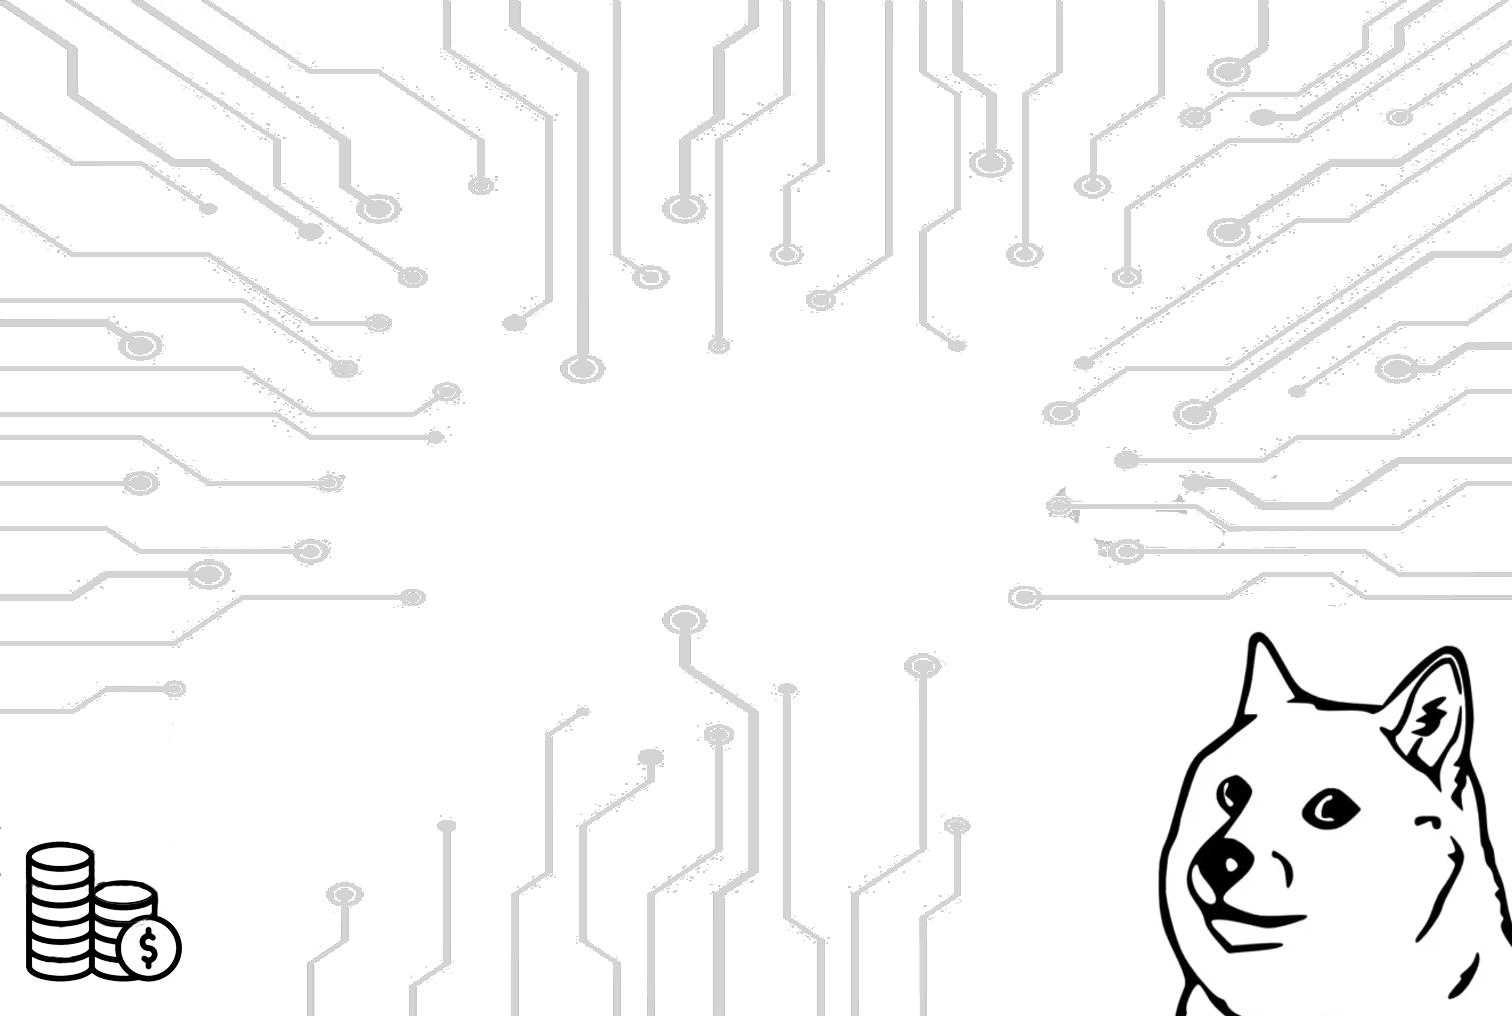
\includegraphics[height=\paperheight,width=\paperwidth]{./images/Background_43_opacity2.png}};}
	
\begin{document}
	
%\section{Início}	

\begin{frame}
	%%%%%%%% Title slide details %%%%%%%%%%%%%%


% Background Image
\newcommand{\myBG}
{
    
\includegraphics[width=\paperwidth]{./images/Background_43_opacity1.jpg}
}

% Title
\newcommand{\myTitle}
{
    %\nohyphenation 
    DO LEGADO AOS CRIPTOATIVOS:\\
    UMA PERSPECTIVA DOS MEIOS DE\\
    PAGAMENTO PARA O ENSINO BÁSICO
}

% Subtitle
\newcommand{\mySubTitle}
{
    Apresentação de trabalho de conclusão de curso\\
    
    {\tiny \url{meet.google.com/jnx-fqge-qvq}}
    
}

% Author
\newcommand{\myAuthor}   
{
    Lucas Herick P. da Silva
    
}

%% Presentation Date
\newdate{PresentationDay}{28}{01}{2022}\ddmmyyyydate 
\date{\displaydate{date}}
\newcommand{\myDate}   
{
    \displaydate{PresentationDay}, \formattime{19}{00}{00}
     
    
}
%
%Logo
\newcommand{\myLogo}   
{
    
\includegraphics[width=.2\textwidth]{./images/uff_main.png}
    \hspace{3mm}
    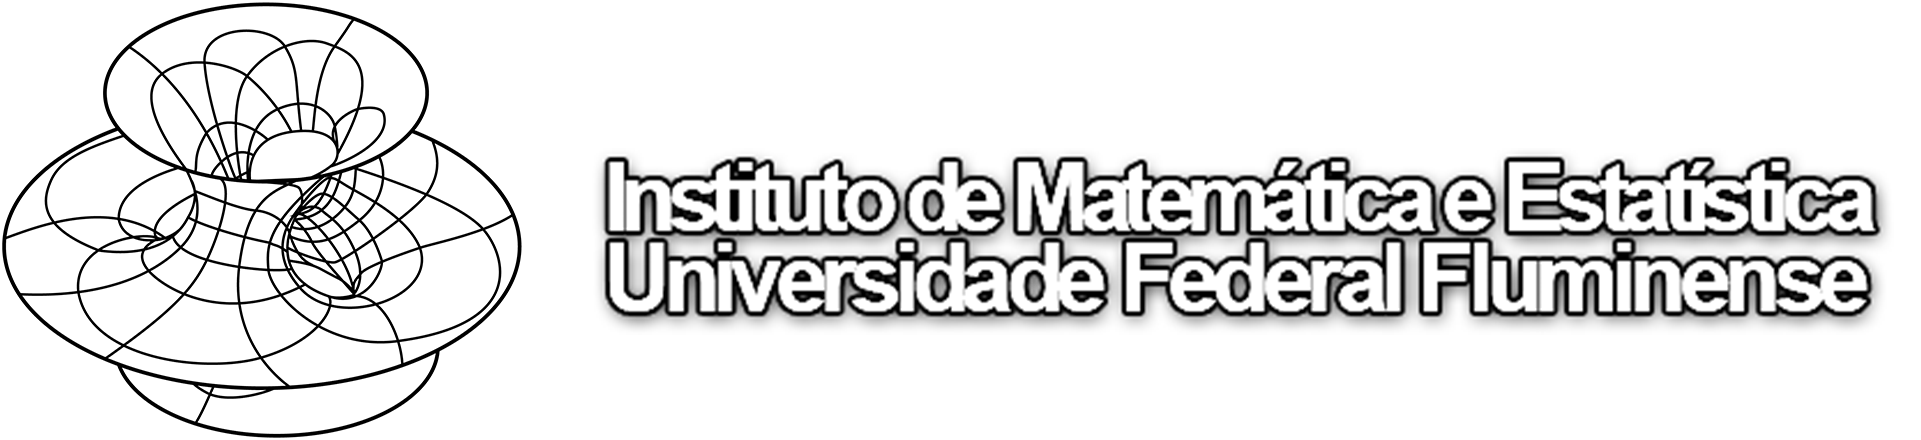
\includegraphics[width=.3\textwidth]{./images/logoescrito3_imeuff.png}
}
%%%%%%%%%%%%%%%%%%%%%%%%%%%%%%%%%%%%


%%%%%%%%%% Title slide code %%%%%%%%%%%
\begin{tikzpicture}[remember picture,overlay]

% Background image
\node[above right,inner sep=0pt] at (current page.south west)
    {
        \myBG
    };
    
% Title & Subtitle
\node
[
    above=0.5cm,
    align=center,
    fill=black!10,
    rounded corners,
    inner xsep=15pt,
    inner ysep=10pt, 
    minimum width=0.7\textwidth,
    text width=0.7\textwidth
] (title) at (current page.center)
{
    \LARGE \myTitle  \\[5pt]
    \small \mySubTitle
};

 Author 
\node[below=0.5cm] (author) at (title.south){\myAuthor};


 Date
\node[below=.5cm] (date) at (author.south){ \myDate};

 Logo
\node
[
    below =0.5cm
] at (date.south)
{
    \myLogo
};

\end{tikzpicture}
\end{frame}	

\section{Sobre}

\begin{frame}
	\frametitle{Sobre o Autor}
	
	\begin{columns}
		
		\column{0.5\linewidth}
				
		\begin{center}
				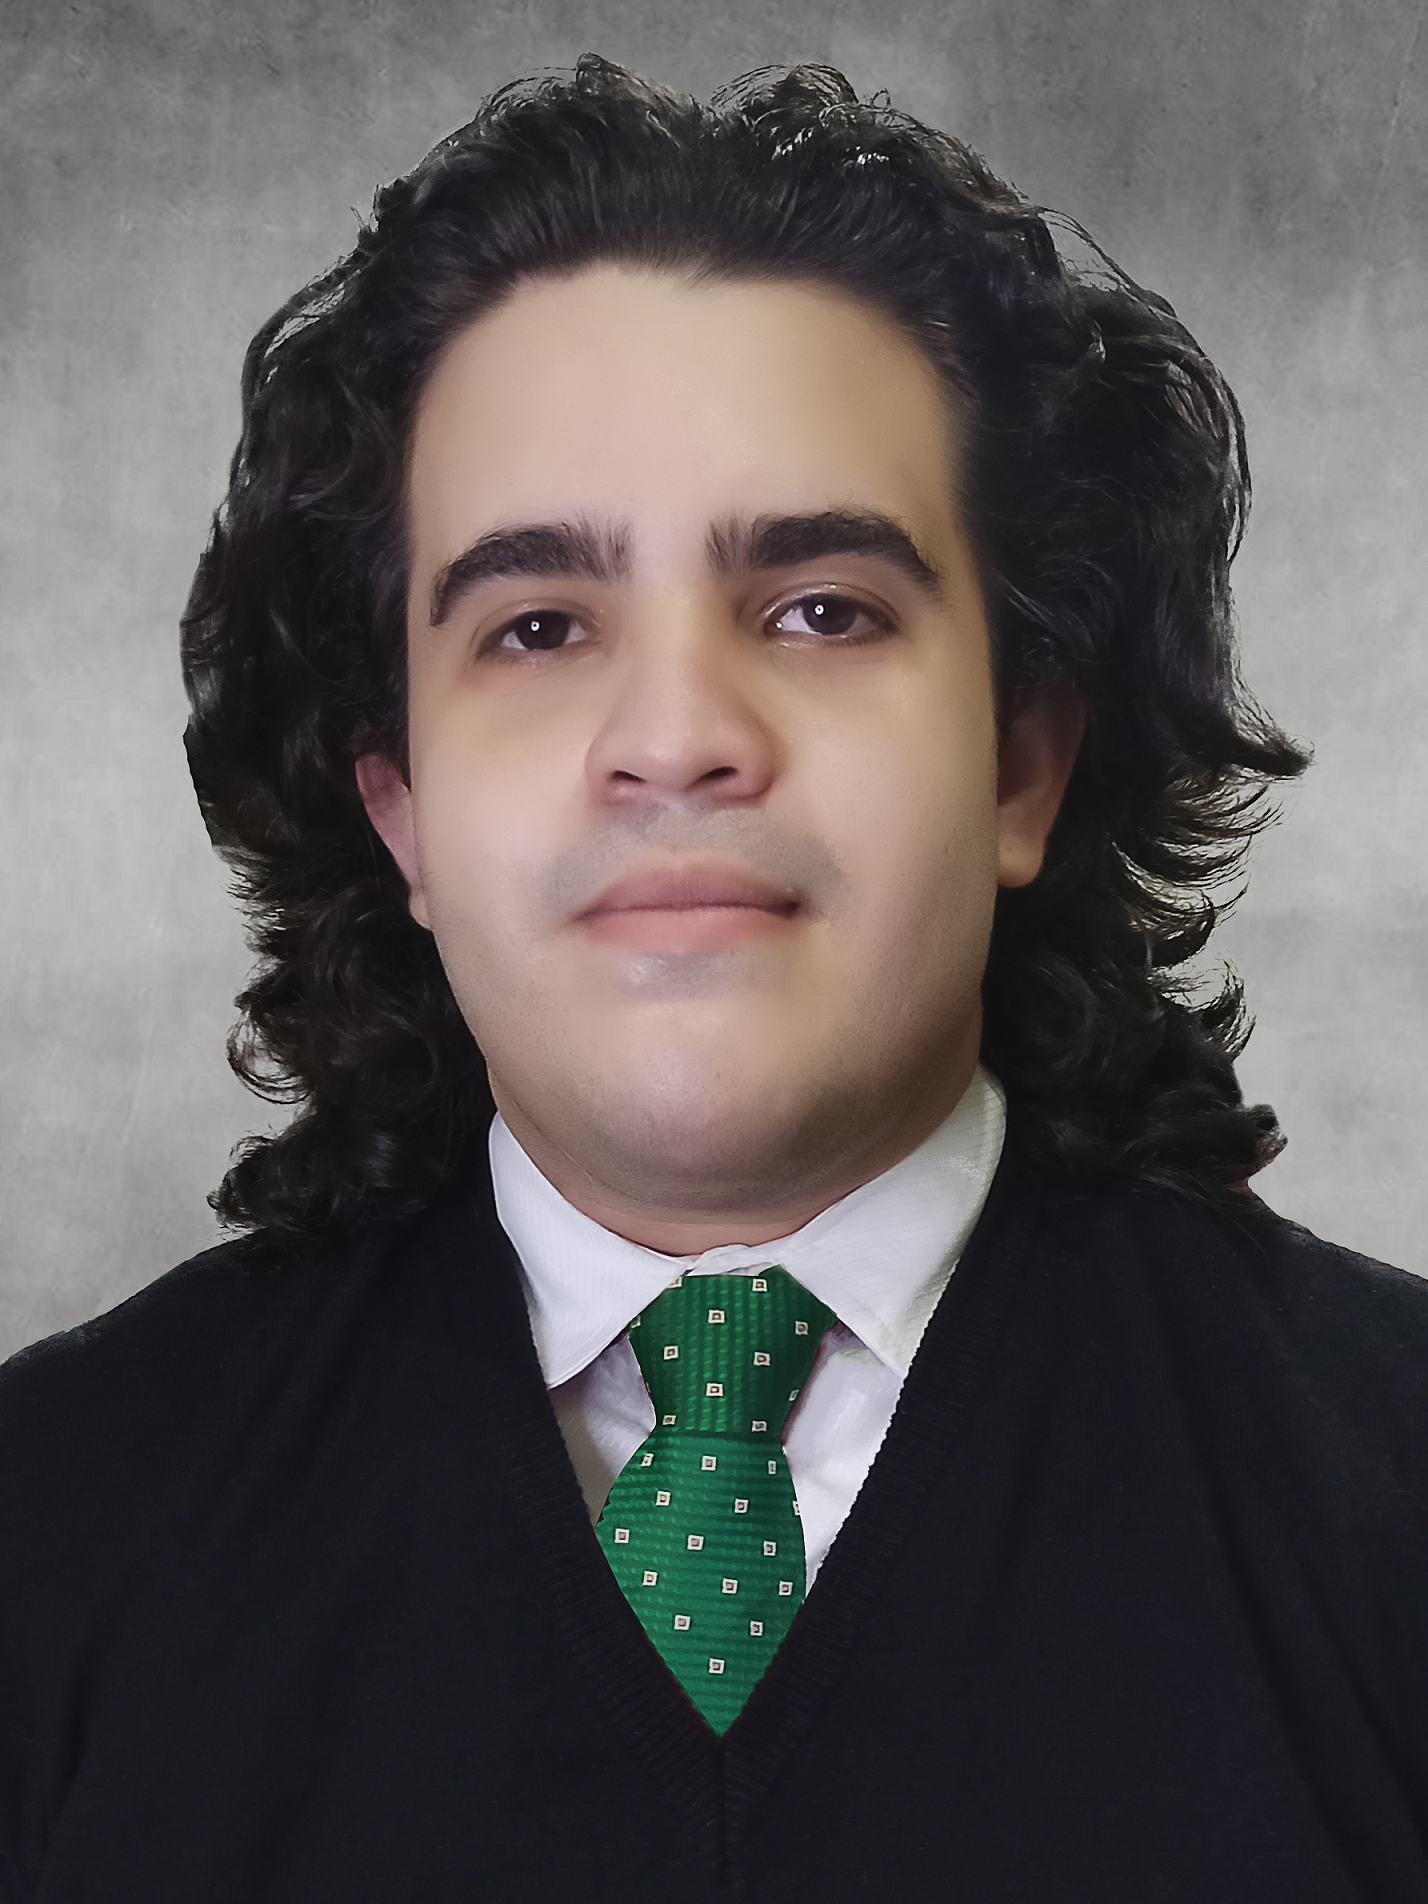
\includegraphics[width = 0.7\linewidth]{LHPS.png}
		\end{center}
			
		\column{0.5\linewidth}
%		
	Lucas Herick Pereira da Silva
	
	\vspace{5mm}
	
		\begin{enumerate}
		\item Analista de desenvolvimento cloud pela Extractta Systems  Technology.
		\item Membro do Centro de Inteligência em Dados (CID) da Alelo Brasil.
		\item Entusiasta em Ciência de Dados, Design Gráfico e Produção musical.
		\end{enumerate}
	
	\begin{figure}
		\centering
		
\includegraphics[width=.3\linewidth]{linkedin_qrcode.png}
		
\includegraphics[width=.3\linewidth]{youtube_qrcode.png}
	\end{figure}
	
	%\begin{center}
	%
\includegraphics[width = 0.3\linewidth, opacity = 0.2]{extractta.png}
	%
\includegraphics[width = 0.3\linewidth]{aws.png}
	%\includegraphics[width = 0.2\linewidth]{alelo.png}
	%\end{center}	
	\end{columns}
\end{frame}

%--------------------FIM DO SOBRE--------------------

\section{Introdução}

\begin{frame}
	\frametitle{Introdução - Citação do capítulo}
	
		\begin{figure}
		\centering
		{\footnotesize Fonte:  \url{https://www.azquotes.com/quote/1020895}}\\
		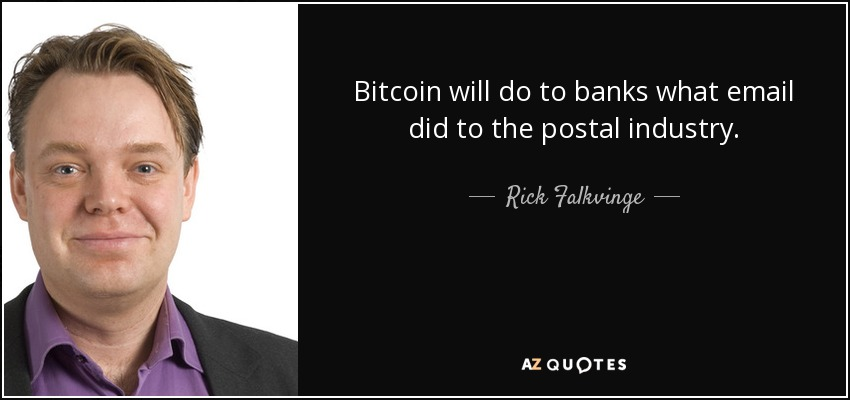
\includegraphics[width = 0.7\linewidth]{quote_intro.jpg}
		\caption{``(O) Bitcoin fará aos bancos o que o e-mail
			fez à indústria postal'' - Rick Falkvinge
			(tradução livre)}
		\end{figure}
\end{frame}

\begin{frame}
	\frametitle{Introdução}
	
	\begin{keypoint}
	
	\begin{enumerate}
		\item Contextualização
%		\begin{itemize}
%			\item Integração \textit{Machine Learning} e \textit{Internet of Things}
%			\item Volatilidade do Bitcoin 
%		\end{itemize}
 \pause
		
		\item Temática 
%		\begin{itemize}
%			\item Referência para citação inicial
%		\end{itemize} 
\pause
		
		\item Objetivos 
%		\begin{itemize}
%			\item Objetivo Geral
%				\begin{itemize}
%					\item Sintetizar a história das transações humanas em um breve contexto histórico e disseminar criptoliteracia que é o conhecimento sobre criptomoedas argumentando sobre suas funções e características na esperança de em algum momento no futuro estes sejam
%					acessíveis e de fácil compreensão, independentemente da renda, status educacional ou sexo. 
%				\end{itemize}\pause
%			\item Objetivos específicos
%		\end{itemize} 
	\end{enumerate}
	\end{keypoint}
		\end{frame}
	
	\begin{frame}
		\frametitle{Introdução}
			\begin{keypoint}
			\begin{enumerate}
				 \setcounter{enumi}{3}
		\item Estruturação do trabalho 
\pause 
		\begin{itemize}
			\item Capítulo 2: Resumo histórico das evoluções de transações e das moedas, como a utilização dos metais, evolução do papel moeda, cartões de débito e crédito até o dinheiro digital. 
			\item Capítulo 3: apresentação sobre o futuro das moedas. É feita uma introdução rápida sobre criptografia, o dinheiro virtual, uma ideia geral sobre o que são as criptomoedas e a percepção geral da população mundial sobre o tema. 
			\item Capítulo 4: Desenvolvimento de atividade sobre custos e ganhos na mineração de criptomoedas e cálculo do tempo de retorno na adquirência de hardware.
			\item Capítulo 5: Conclusão e sugestões de trabalhos futuros. 
		\end{itemize}
\pause
	\item Relevância do trabalho
%			\begin{itemize}
%				\item Relato da aproximação do autor com o tema. 
%			\end{itemize} 
		
		
	\end{enumerate}
	\end{keypoint}
\end{frame}

%--------------------FIM DO CAP 1--------------------

\section{Histórico}

\begin{frame}
	\frametitle{Histórico - Citação do capítulo}
	
	\begin{figure}
		\centering
		{\footnotesize Fonte:  \url{https://bit.ly/3mF31a7}}\\
		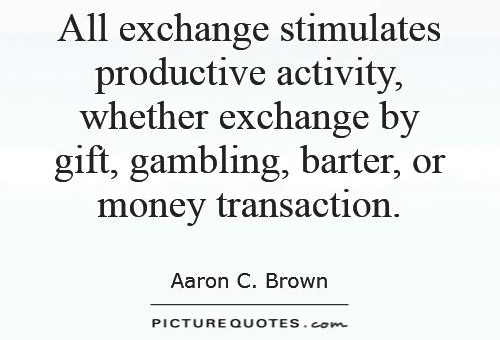
\includegraphics[width = 0.5\linewidth]{quote_chap2.jpg}
		\caption{
			``Toda troca estimula a atividade produtiva,
			seja troca por presente, aposta, escambo ou
			transação com dinheiro.'' - Aaron C. Brown
			(tradução livre)
}
	\end{figure}
\end{frame}

\begin{frame}<1>[label=chap2]
	\frametitle{Histórico}
		\begin{keypoint}
		
		\begin{enumerate}
			\item Prólogo
%			\begin{itemize}
%				\item Condução do leitor para período pre-histórico
%			\end{itemize}
\pause
			
			\item O princípio 
%			\begin{itemize}
%				\item Escambo
%				\item Conchas (e outros objetos)
%			\end{itemize} 

\pause
			
			\item Metais 
%			\begin{itemize}
%				\item Cunhagem
%				\item Primeira moeda oficial
%			\end{itemize}
\pause
			\item Transição para o papel moeda 
\pause
			\item Guerras cambiais 
\pause
			\item Cartões e ATMs 	
\pause
		
			\item Transações eletrônica e bancos digitais 
		\end{enumerate} 
	\end{keypoint}
\end{frame}

\begin{frame}[noframenumbering]
	\begin{figure}
		\centering
		{\footnotesize Fonte: Desenvolvido pelo com assets open-source e plataforma whimsical}\\
		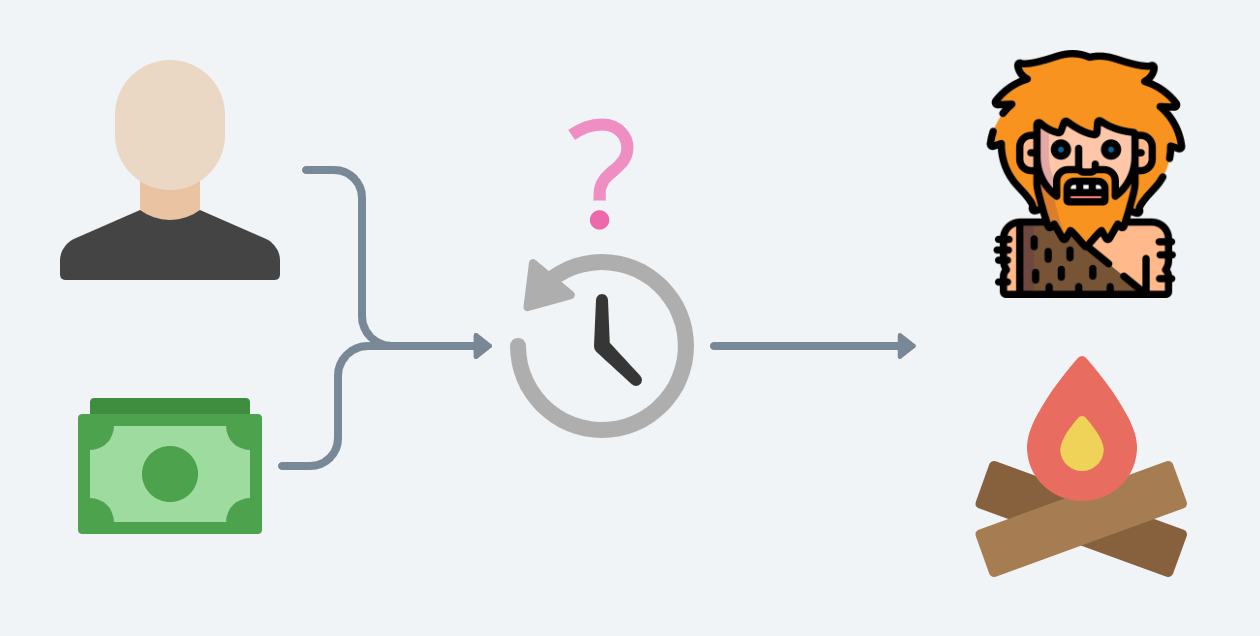
\includegraphics[width = 0.8\linewidth]{time_travel.png}
		\caption{}
	\end{figure}
\end{frame}
\againframe<2>{chap2}
\begin{frame}[noframenumbering]
	\begin{figure}
		\centering
		{\footnotesize Fonte: Utilizado no documento}\\
		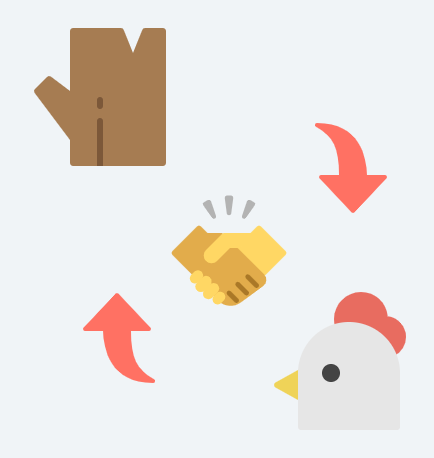
\includegraphics[width = 0.35\linewidth]{barter_1.png}
		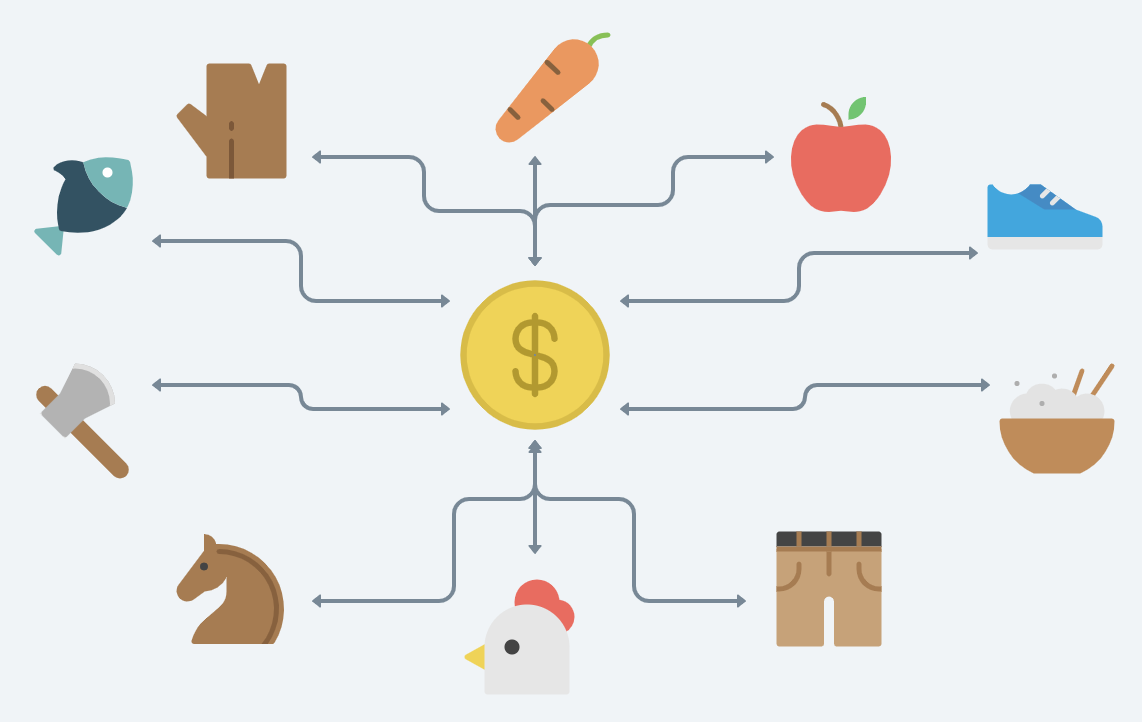
\includegraphics[width = 0.57\linewidth]{barter_2.png}
		\caption{}
	\end{figure}
\end{frame}
\againframe<3>{chap2}
\begin{frame}[noframenumbering]
	\begin{figure}
		\centering
		{\footnotesize Fonte: Utilizadas no documento}\\
		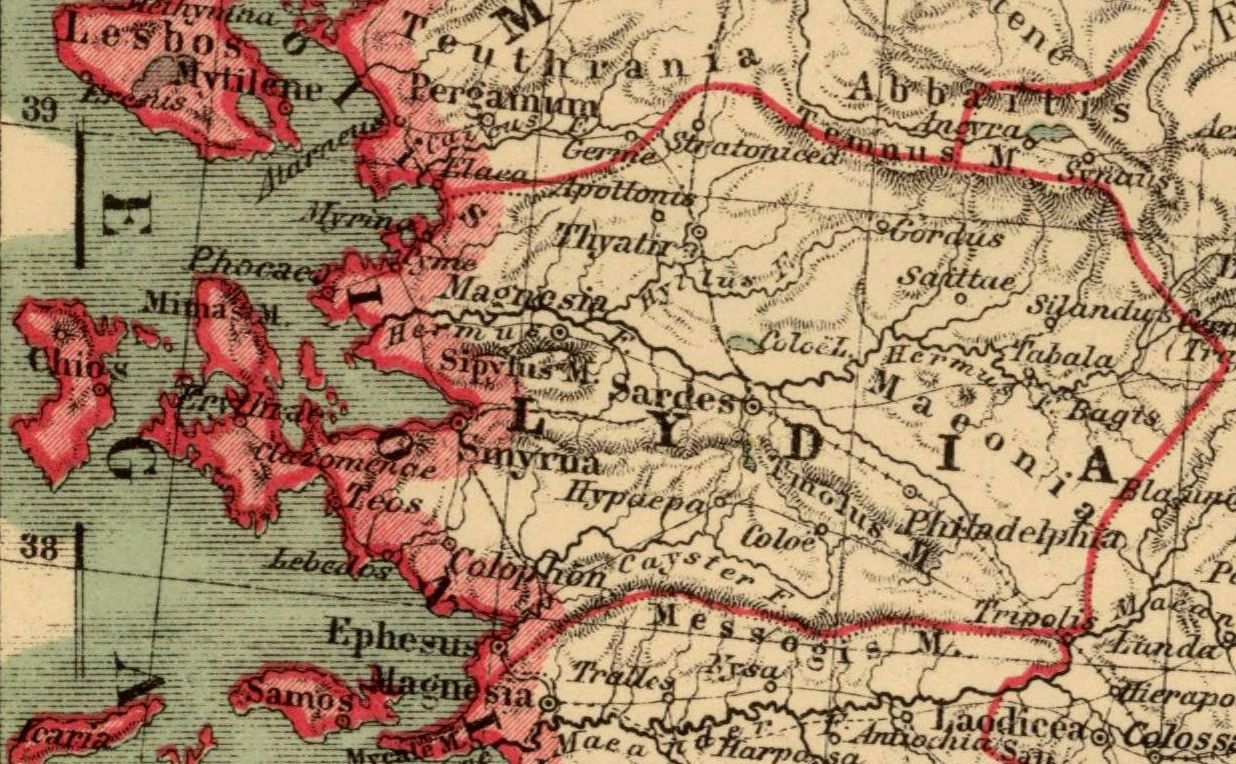
\includegraphics[width = 0.45\linewidth]{Lydia_map.jpg}
		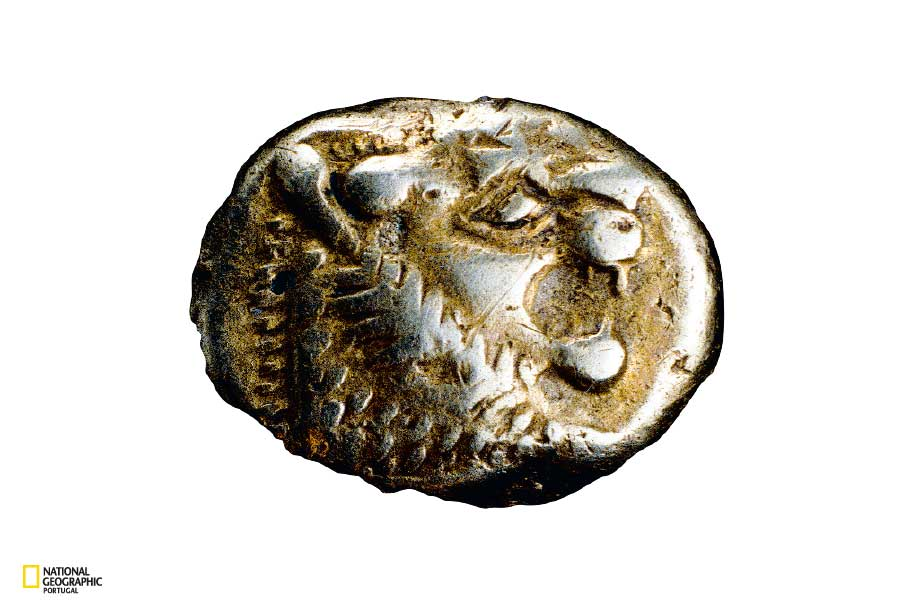
\includegraphics[width = 0.50\linewidth]{lydian_lion.jpg}
		\caption{}
	\end{figure}
\end{frame}
\againframe<4>{chap2}
\begin{frame}[noframenumbering]
	\begin{figure}
		\centering
		{\footnotesize Fonte: Utilizado no documento}\\
		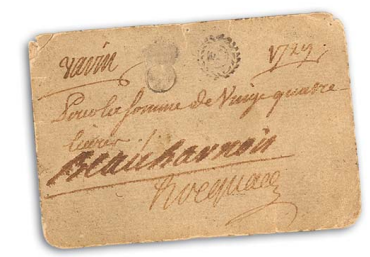
\includegraphics[width = 0.4\linewidth]{card_money.png}
		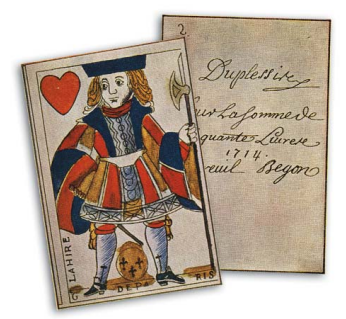
\includegraphics[width = 0.4\linewidth]{card_money2.png}
		\caption{}
	\end{figure}
\end{frame}
\againframe<5>{chap2}
%\begin{frame}[noframenumbering]
%	picture5
%\end{frame}
\againframe<6>{chap2}
\begin{frame}[noframenumbering]
	\begin{figure}
		\centering
		{\footnotesize Fonte: \url{https://bit.ly/3qPp943}}\\
		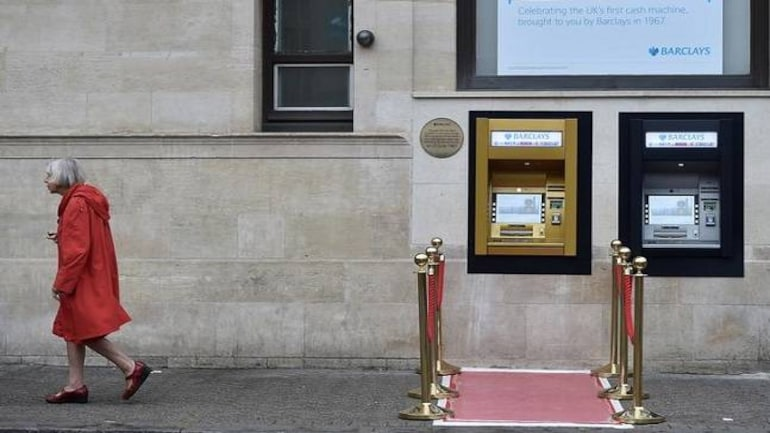
\includegraphics[width = 0.8\linewidth]{the_first_atm.jpg}
		\caption{}
	\end{figure}
\end{frame}
\againframe<7>{chap2}
\begin{frame}[noframenumbering]
		\begin{figure}
		\centering
		{\footnotesize Fonte: Utilizado no documento}\\
		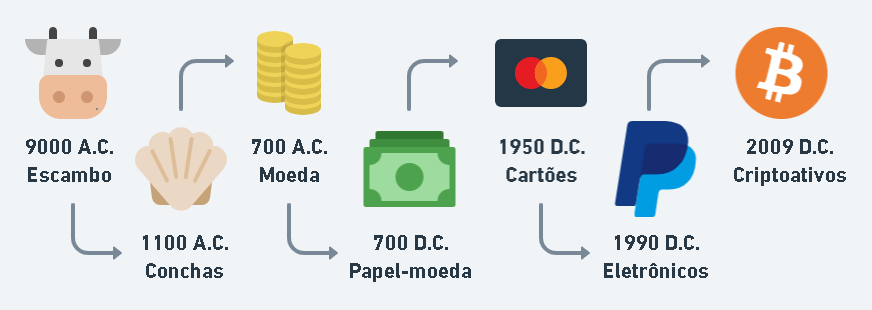
\includegraphics[width = 0.8\linewidth]{Resumo.png}
		\caption{}
	\end{figure}
\end{frame}
%--------------------FIM DO CAP 2--------------------

\section{O futuro}

\begin{frame}
	\frametitle{O futuro - Citação do capítulo}
	
		\begin{figure}
		\centering
		{\footnotesize Fonte:  \url{https://www.azquotes.com/quote/1030064}}\\
		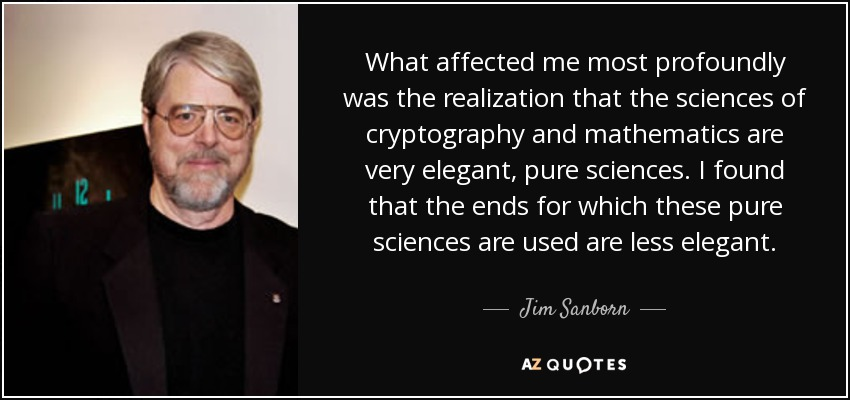
\includegraphics[width = 0.7\linewidth]{quote_chap3.jpg}
		\caption{``O que me afetou mais profundamente foi a
			percepção de que as ciências da criptografia e
			da matemática são ciências puras muito
			elegantes. Descobri que os fins para os quais
			essas ciências puras são usadas são menos
			elegantes.'' -  Jim Sanborn
			(tradução livre)}
	\end{figure}
\end{frame}

\begin{frame}<1>[label=chap3]
	\frametitle{O futuro}
	\begin{keypoint}
		
		\begin{enumerate}
			\item Noções de criptografia 
%			\begin{itemize}
%				\item Ideia geral
%				\item Métodos criptográficos históricos
%				\item Chaves criptográficas
%				\item Blockchain
%			\end{itemize}
\pause			
			\item Criptoativos 
%			\begin{itemize}
%				\item Conceito
%				\item Concepção
%				\item Receptividade no mundo e na sociedade brasileira
%				\item Proposta de questionário
%			\end{itemize} 
			
		\end{enumerate} 
	\end{keypoint}
\end{frame}

\begin{frame}[noframenumbering]
	\begin{figure}
		\centering
		{\footnotesize Fonte: Utilizado no documento}\\
		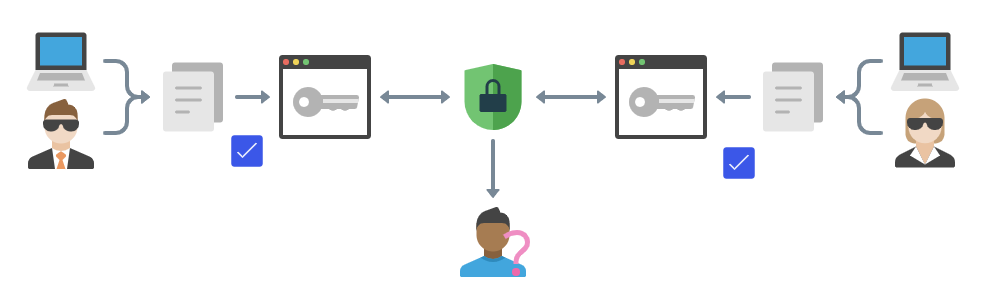
\includegraphics[width = 0.95\linewidth]{Private-Public_Key.png}
		\caption{Esquema de funcionamento das criptografias por chave pública e por chave privada}
	\end{figure}
\end{frame}
\againframe<2>{chap3}
\begin{frame}[noframenumbering]
\begin{figure}
	\centering
	{\footnotesize Fonte: (AGÊNCIA DINO, 2021)}\\
	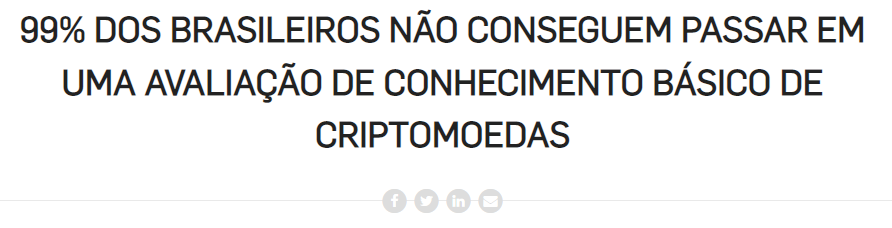
\includegraphics[width = 0.95\linewidth]{teste_crypto.png}
	\caption{Esquema de funcionamento das criptografias por chave pública e por chave privada}
\end{figure}
\end{frame}


%--------------------FIM DO CAP 3--------------------

\section{Atividade}

\begin{frame}
	\frametitle{Atividade - Citação do capítulo}
	
	\begin{figure}
		\centering
		{\footnotesize Fonte:  \url{https://www.bitcoinersanonymous.com/project/abigail-johnson/}}\\
		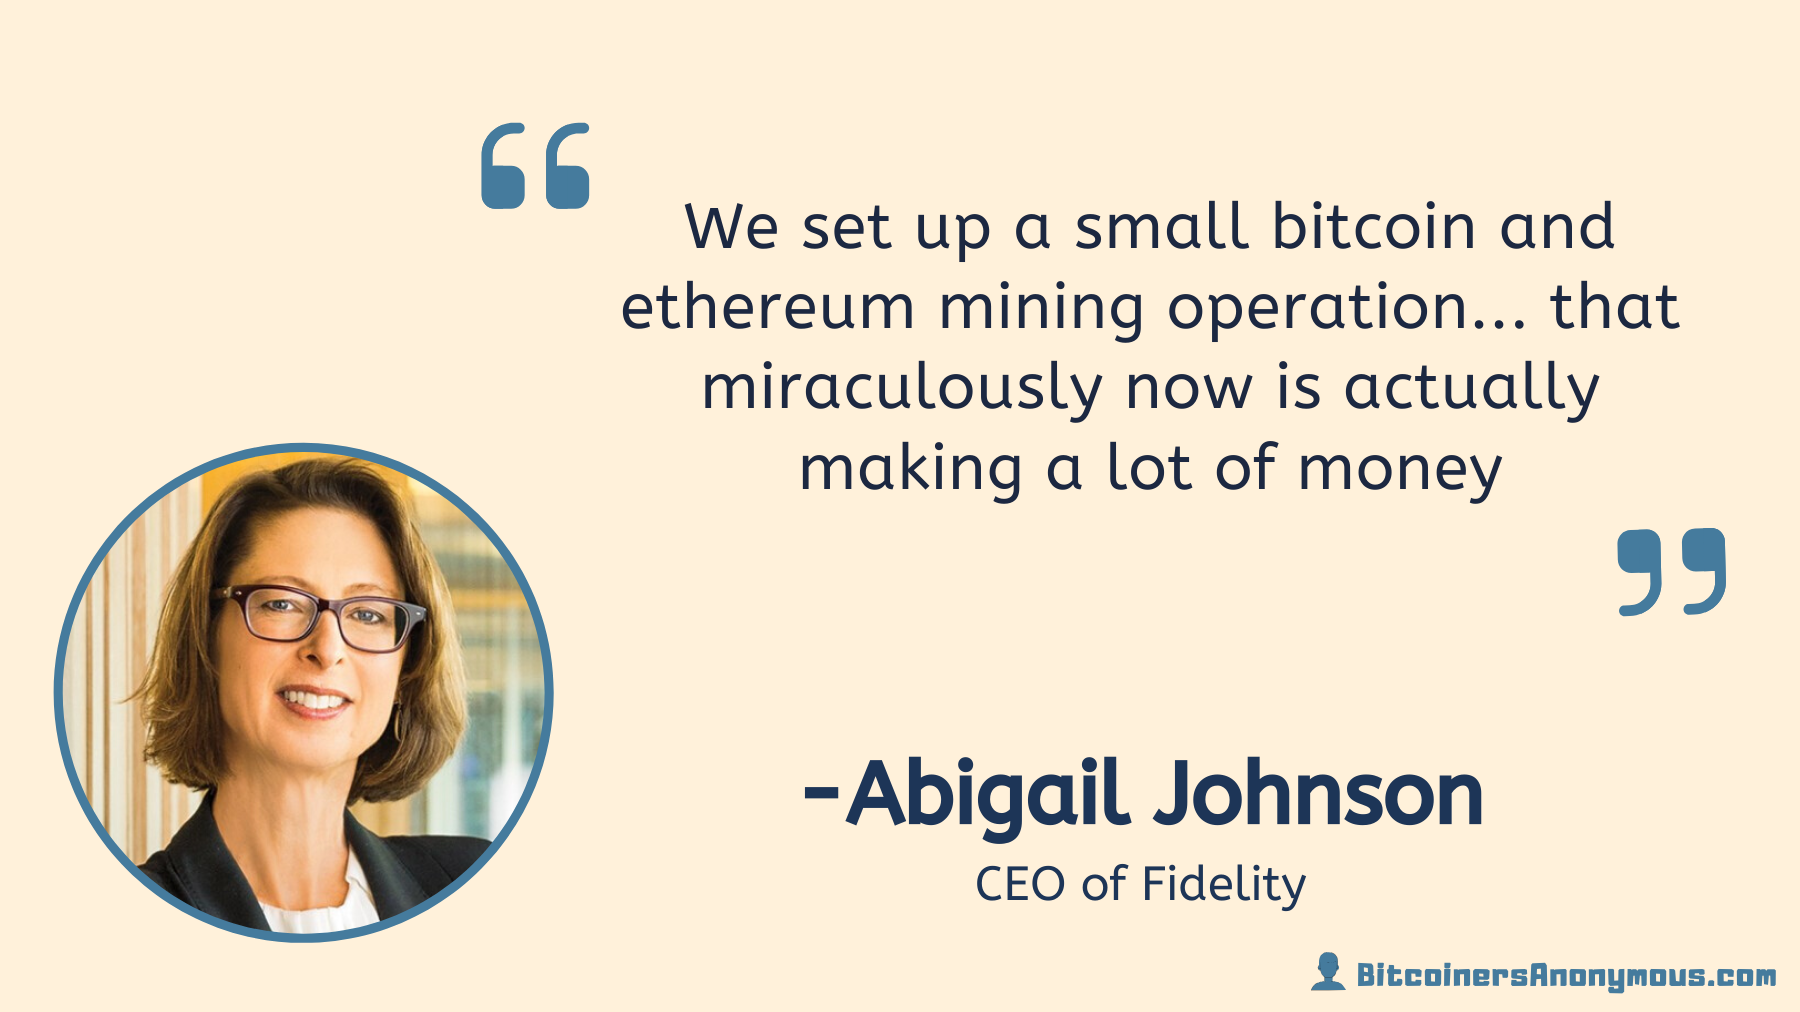
\includegraphics[width = 0.7\linewidth]{quote_chap4.jpg}
		\caption{``Montamos uma pequena operação de
			mineração de bitcoin e ethereum... que
			milagrosamente agora está ganhando muito
			dinheiro'' - Abigail Johnson
			(tradução livre)}
	\end{figure}
\end{frame}

\begin{frame}<1>[label=chap4p1]
	\frametitle{Atividade}
	\begin{keypoint}
		
		\begin{enumerate}
			\item Introdução 
%				\begin{itemize}
%					\item Motivador
%				\end{itemize}
\pause
			\item Embasamento 	
%				\begin{itemize}
%					\item Bases conceituais
%					\begin{itemize}
%						\item Matemátia financeira
%						\item Conversões de medidas
%					\end{itemize}
\pause
			%	\end{itemize}
					\item Construção 
%						\begin{itemize}
%							\item Habilidades BNCC 
%						\end{itemize} 
\pause
					\item Infraestruturas digitais
%					\begin{itemize}
%						\item On premise versus cloud
%						\item Sistemas operacionais
%					\end{itemize} 
\pause
%				\end{itemize}
		\end{enumerate} 
	\end{keypoint}
\end{frame}

\begin{frame}[noframenumbering]
	\begin{figure}
		\centering
		{\footnotesize Fonte: Utilizado no documento}\\
		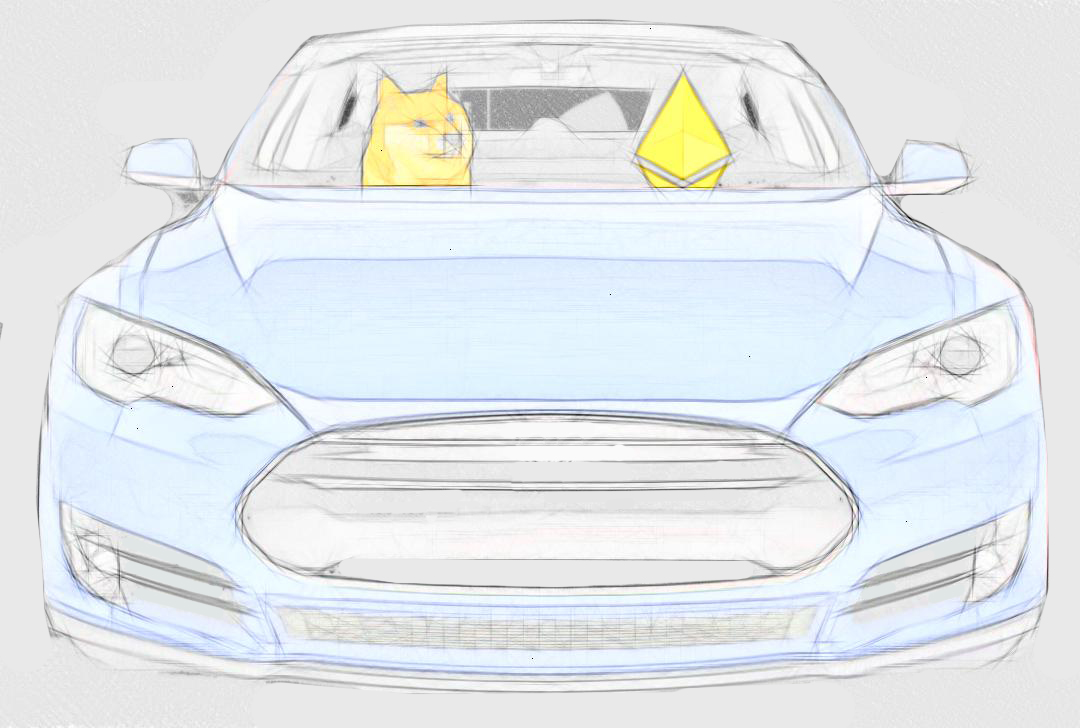
\includegraphics[width = 0.7\linewidth]{tesla-ethereum-doge_sketch.jpg}
		\caption{Um passeio veicular}
	\end{figure}
\end{frame}
\againframe<2>{chap4p1}
%\begin{frame}[noframenumbering]
%	picture2.1
%\end{frame}
\againframe<3>{chap4p1}
\begin{frame}[noframenumbering]
	\begin{figure}
		\centering
		{\footnotesize Fonte: Print do documento}\\
		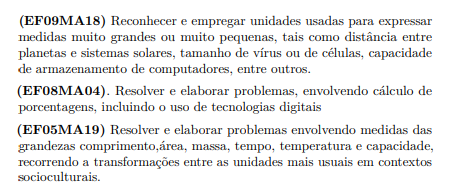
\includegraphics[width = 0.7\linewidth]{BNCC.png}
		\caption{BNCC - Habilidade visadas}
	\end{figure}
\end{frame}
\againframe<4>{chap4p1}
\begin{frame}[noframenumbering]
	\begin{figure}
		\centering
		{\footnotesize Fonte: \url{https://www.micromata.de/blog/on-premise-vs-cloud/}}\\
		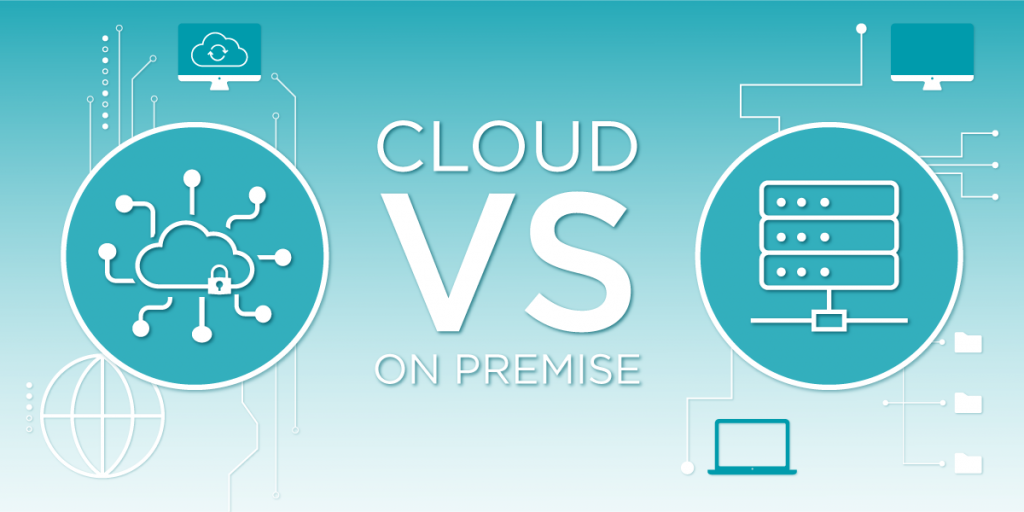
\includegraphics[width = 0.7\linewidth]{on_premise_cloud.png}
		\caption{On premise versus cloud}
	\end{figure}
\end{frame}

\begin{frame}<1>[label=chap4p2]
	\frametitle{Atividade}
	\begin{keypoint}
		
		\begin{enumerate}
			\setcounter{enumi}{4}
			\item Guia do professor
%			\begin{itemize}
%				\item Planilha piloto
%			\end{itemize} 
\pause
			
			\item Plano de aula 
%			\begin{itemize}
%				\item Materiais necessários
%				\item Metodologia
%				\item Avaliação
%			\end{itemize} 
\pause
			
			\item Exemplo de resultado \pause
			 
		\end{enumerate} 
	\end{keypoint}
\end{frame}
%\begin{frame}[noframenumbering]
%	picture3
%\end{frame}
\againframe<2>{chap4p2}
%\begin{frame}[noframenumbering]
%	picture4
%\end{frame}
\againframe<3>{chap4p2}
%\begin{frame}[noframenumbering]
%	picture5
%\end{frame}



%--------------------FIM DO CAP 4--------------------

\section{Considerações}

\begin{frame}
	\frametitle{Considerações Finais - Citação do capítulo}
	
	\begin{figure}
		\centering
		{\footnotesize Fonte:  \url{https://biblics.com/en/bible/good-news-bible-anglicised/old-testament/ecclesiastes/11/1}}\\
		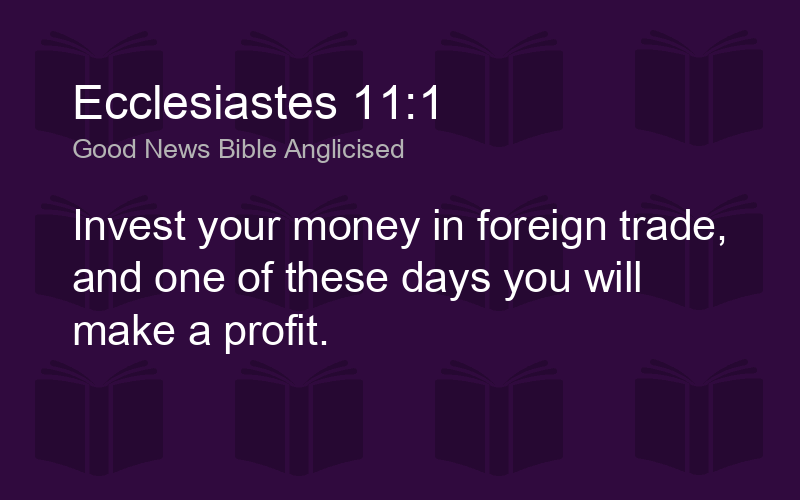
\includegraphics[width = 0.7\linewidth]{quote_chap5.jpg}
		\caption{``Invista seu dinheiro no comércio exterior, e
			um dia desses você terá lucro.'' - Bíblia Sagrada, edição boas novas anglicizada.
			(tradução livre)}
	\end{figure}
\end{frame}

\begin{frame}
	\frametitle{Considerações Finais}
	\begin{keypoint}
		
		\begin{enumerate}
			\item Conclusões 
			\item Sugestões para trabalhos futuros
		\end{enumerate} 
	\end{keypoint}
\end{frame}

\section{Final}

\begin{frame}
	\frametitle{Final }
	
	\begin{center}
	{\Huge Q\&A}
	
	\vspace{5mm}
	
	(Perguntas e respostas)
	\end{center}

\end{frame}
\begin{frame}
	\frametitle{Final}
%	Meus sinceros agradecimentos para:
%	
%	\vspace{5mm}
%	
%{\small 	\begin{itemize}
%		\item A todos aqueles que estão presentes nesta apresentação
%		\item A todos citados na seção de agradecimentos no documento. 
%	\end{itemize}}
%
%\vspace{1cm}

\noindent
\begin{center}
	{\Huge Obrigado.\\
		   Thank you.\\
		   Merci. \\
		   Gracias.\\ 
		   \vspace{3mm} $\underset{{\text{\footnotesize(gamsahamnida)}}}{\text{감사합니다}}$.}
\end{center}

\end{frame}

%-----------------------------------------------
\end{document}